% SC4051 --- Chapter 6: Distributed Storage (0->100)
\chapter{Distributed Storage: Files, Blocks and Objects}
\label{ch:storage}

\begin{quote}
\emph{``A file system is a database with a funny API; a distributed file system is a database that must also survive partitions.''} We layer that idea from files to blocks to objects.
\end{quote}

\noindent\fbox{\parbox{\dimexpr\linewidth-2\fboxsep-2\fboxrule}{%
\textbf{From zero: what ``storing a file'' means when disks are remote.} We start with a local file, make the disk remote, then replicate and stripe it. We contrast file, block and object abstractions and study HDFS and S3 as canonical designs.}}
\vspace{0.4em}

\section*{Learning Outcomes}
After this chapter you will be able to:
\begin{enumerate}[label=(L\arabic*)]
    \item distinguish file, block and object storage on interface, mutability and scale;
    \item explain HDFS architecture (NameNode, DataNodes, blocks, replication, rack awareness);
    \item describe S3's key model, consistency, multipart upload and lifecycle;
    \item compare striping/erasure coding vs.\ replication on overhead and recovery;
    \item reason about metadata scaling (NameNode bottleneck) and its mitigations.
\end{enumerate}

% ============================================================
\section{Three Abstractions}
\label{sec:abstractions}
\begin{description}[leftmargin=1.2em,style=nextline]
    \item[File storage] Hierarchical namespace (directories, files), POSIX-like operations, byte-range reads/writes, strong consistency per file. Examples: NFS, HDFS, GFS.
    \item[Block storage] Raw fixed-size blocks addressed by block ID, no files or directories; the OS formats a filesystem on top. Examples: EBS, Ceph RBD.
    \item[Object storage] Flat namespace of variable-size immutable objects addressed by key (bucket/key), rich metadata, HTTP API, massive scale, eventual or read-after-write consistency. Examples: S3, GCS, Azure Blob.
\end{description}

Files suit shared POSIX workloads; blocks suit databases that manage their own layout; objects suit web-scale, write-once, read-many data (images, logs, backups) where scale and durability trump POSIX semantics.

\begin{figure}[h]
\centering
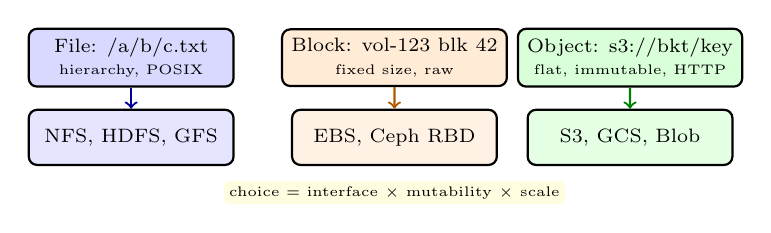
\begin{tikzpicture}[scale=0.88, every node/.style={font=\scriptsize},
  box/.style={draw,rounded corners=3pt,minimum width=2.6cm,minimum height=0.70cm,align=center,thick}]
\node[box,fill=blue!15] (file) at (0,1.7) {File: /a/b/c.txt\\{\tiny hierarchy, POSIX}};
\node[box,fill=orange!16] (block) at (3.8,1.7) {Block: vol-123 blk 42\\{\tiny fixed size, raw}};
\node[box,fill=green!15] (obj) at (7.2,1.7) {Object: s3://bkt/key\\{\tiny flat, immutable, HTTP}};
\node[box,fill=blue!10] (f2) at (0,0.55) {NFS, HDFS, GFS};
\node[box,fill=orange!10] (b2) at (3.8,0.55) {EBS, Ceph RBD};
\node[box,fill=green!10] (o2) at (7.2,0.55) {S3, GCS, Blob};
\draw[->,thick,blue!60!black] (file) -- (f2);
\draw[->,thick,orange!70!black] (block) -- (b2);
\draw[->,thick,green!50!black] (obj) -- (o2);
\node[font=\tiny,fill=yellow!12,rounded corners=2pt,inner sep=2pt] at (3.8,-0.25) {choice = interface $\times$ mutability $\times$ scale};
\end{tikzpicture}
\caption{Three storage abstractions. Moving right trades POSIX mutability for scale and simplicity.}
\label{fig:abstractions}
\end{figure}

% ============================================================
\section{HDFS: A Distributed File System}
\label{sec:hdfs}
The Hadoop Distributed File System (HDFS) stores very large files as a sequence of fixed-size \emph{blocks} (default 128\,MB). Architecture:

\begin{description}[leftmargin=1.2em,style=nextline]
    \item[NameNode] Holds the namespace, file-to-block mapping and block locations---all in RAM. The single metadata bottleneck.
    \item[DataNodes] Store blocks on local disks, report block lists (block reports) and heartbeats to the NameNode.
    \item[Client] Asks NameNode for block locations, then reads/writes directly to DataNodes (data path bypasses NameNode).
\end{description}

Replication (default $3\times$) is rack-aware: replica 1 on the writer's rack, replica 2 on a different rack, replica 3 on the same rack as replica 2---survives one node and one rack failure. Writes are pipelined through the replica chain (as in Ch.~5). HDFS trades POSIX completeness for throughput: write-once, append-possible, no random writes, optimised for streaming reads.

\begin{figure}[h]
\centering
\begin{tikzpicture}[scale=0.86, every node/.style={font=\scriptsize},
  box/.style={draw,rounded corners=3pt,minimum width=2.0cm,minimum height=0.70cm,align=center,thick}]
\node[box,fill=red!15] (nn) at (3.6,2.4) {NameNode\\{\tiny namespace, block map}};
\node[box,fill=blue!14] (client) at (0,2.4) {Client};
\node[box,fill=green!14] (dn1) at (0,0.95) {DataNode 1\\{\tiny blk\_A1, blk\_B2}};
\node[box,fill=green!14] (dn2) at (3.6,0.95) {DataNode 2\\{\tiny blk\_A2, blk\_C1}};
\node[box,fill=green!14] (dn3) at (7.0,0.95) {DataNode 3\\{\tiny blk\_A3, blk\_B1}};
\draw[->,thick,blue!60!black] (client) -- (nn) node[midway,above,font=\tiny] {where is /file?};
\draw[<-,thick,orange!70!black] (nn) -- (dn1) node[midway,left,font=\tiny] {heartbeat};
\draw[<-,thick,orange!70!black] (nn) -- (dn2);
\draw[<-,thick,orange!70!black] (nn) -- (dn3);
\draw[->,thick,green!50!black] (client) -- (dn1) node[midway,left,font=\tiny] {data};
\draw[->,thick,green!50!black] (client) to[bend right=10] (dn2);
% rack boxes
\begin{scope}[on background layer]
  \fill[blue!6,rounded corners=4pt] (-0.95,0.30) rectangle (2.1,1.60);
  \fill[orange!6,rounded corners=4pt] (2.8,0.30) rectangle (7.9,1.60);
\end{scope}
\node[font=\tiny] at (0.55,0.40) {Rack 1}; \node[font=\tiny] at (5.35,0.40) {Rack 2};
\end{tikzpicture}
\caption{HDFS: NameNode holds metadata; clients stream data directly to/from DataNodes. Replication is rack-aware.}
\label{fig:hdfs}
\end{figure}

\paragraph{NameNode scale.} The NameNode keeps $\approx 150$ bytes per block in RAM; a 100M-block cluster needs $\sim$15\,GB just for block metadata. Mitigations: HDFS Federation (multiple NameNodes for different namespaces), NameNode HA (active--standby with shared journal), and specialised metadata stores (HopsFS replaces the heap with a NewSQL DB).

% ============================================================
\section{Object Storage and S3}
\label{sec:s3}
Amazon S3 presents a flat key space: each object lives at \texttt{s3://bucket/key} with size up to 5\,TB, metadata, and optional versioning. There are no directories---slashes in keys are a console fiction. Objects are immutable: overwrite creates a new version.

\paragraph{Consistency.} S3 now provides strong read-after-write for new puts and strong read-after-update/delete (since Dec 2020)---earlier it was eventual for overwrites. Listing remains eventually consistent. Multipart upload splits a large object into parts uploaded in parallel and assembled server-side, enabling resume and high throughput.

\paragraph{Durability and lifecycle.} S3 promises $11$ nines durability via cross-AZ replication and erasure coding internally. Lifecycle rules transition objects through storage classes (Standard $\to$ IA $\to$ Glacier) and expire them.

\begin{figure}[h]
\centering
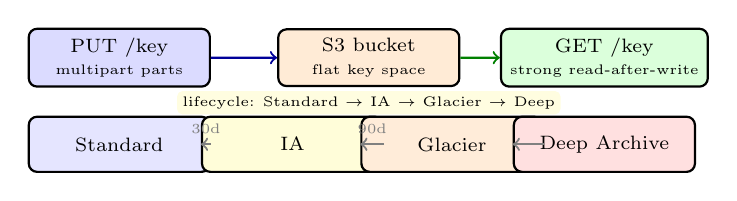
\begin{tikzpicture}[scale=0.88, every node/.style={font=\scriptsize},
  box/.style={draw,rounded corners=3pt,minimum width=2.3cm,minimum height=0.70cm,align=center,thick}]
\node[box,fill=blue!14] (put) at (0,1.6) {PUT /key\\{\tiny multipart parts}};
\node[box,fill=orange!16] (s3) at (3.6,1.6) {S3 bucket\\{\tiny flat key space}};
\node[box,fill=green!14] (get) at (7.0,1.6) {GET /key\\{\tiny strong read-after-write}};
\node[box,fill=blue!10] (std) at (0,0.35) {Standard};
\node[box,fill=yellow!15] (ia) at (2.5,0.35) {IA};
\node[box,fill=orange!15] (gl) at (4.8,0.35) {Glacier};
\node[box,fill=red!12] (deep) at (7.0,0.35) {Deep Archive};
\draw[->,thick,blue!60!black] (put) -- (s3);
\draw[->,thick,green!50!black] (s3) -- (get);
\draw[->,thick,gray] (std) -- (ia) node[midway,above,font=\tiny] {30d};
\draw[->,thick,gray] (ia) -- (gl) node[midway,above,font=\tiny] {90d};
\draw[->,thick,gray] (gl) -- (deep);
\node[font=\tiny,fill=yellow!12,rounded corners=2pt,inner sep=2pt] at (3.6,0.95) {lifecycle: Standard $\to$ IA $\to$ Glacier $\to$ Deep};
\end{tikzpicture}
\caption{S3 object lifecycle and multipart upload. Keys are flat; lifecycle rules automate cost optimisation.}
\label{fig:s3}
\end{figure}

\begin{lstlisting}[language=Python]
# S3-style multipart upload and HDFS block placement (illustrative)
import hashlib, os

# --- S3 multipart: split, hash each part, reassemble ---
def multipart_split(data: bytes, part_size: int = 5):
    parts = [data[i:i+part_size] for i in range(0, len(data), part_size)]
    etags = [hashlib.md5(p).hexdigest() for p in parts]
    # server reassembles in order; overall ETag is hash of concatenated part hashes
    overall = hashlib.md5(b"".join(bytes.fromhex(e) for e in etags)).hexdigest()
    return list(zip(etags, parts)), overall

data = b"Hello distributed storage world!"
parts, etag = multipart_split(data, part_size=8)
print(f"{len(parts)} parts, overall ETag~{etag[:12]}...")
reassembled = b"".join(p for _, p in parts)
assert reassembled == data

# --- HDFS rack-aware replica placement ---
racks = {"dn1":"rack1", "dn2":"rack1", "dn3":"rack2", "dn4":"rack2", "dn5":"rack3"}
def place_replicas(writer_dn, n=3):
    # replica 1: writer's rack, replica 2: different rack, replica 3: same rack as 2
    writer_rack = racks[writer_dn]
    other_racks = [d for d,r in racks.items() if r != writer_rack]
    replica2 = other_racks[0]
    same_rack_as_2 = [d for d,r in racks.items() if r==racks[replica2] and d!=replica2][0]
    return [writer_dn, replica2, same_rack_as_2]

print("placement for writer dn1:", place_replicas("dn1"))
\end{lstlisting}

% ============================================================
\section{Replication vs.\ Erasure Coding}
\label{sec:ec}
$3\times$ replication costs $200\%$ overhead. \emph{Erasure coding} (e.g., Reed--Solomon $k$ data + $m$ parity) tolerates $m$ failures with overhead $m/k$. HDFS EC with $6+3$ uses $50\%$ overhead vs.\ $200\%$ for $3\times$---a $4\times$ saving. The trade-off is recovery cost: reconstructing a lost block needs $k$ other blocks (more I/O and CPU) and small random reads become expensive.

Hence tiered strategies: hot data stays replicated for fast degraded reads; cold data is EC-encoded for capacity. S3, GFS and Ceph all tier this way.

\begin{lstlisting}[language=Python]
# Erasure coding vs replication: storage overhead and fault tolerance
def overhead(replicas=None, k=None, m=None):
    if replicas: return (replicas - 1) * 100  # percent extra
    return m / k * 100

print(f"3x replication overhead: {overhead(replicas=3):.0f}%")
for k,m in [(6,3),(10,4),(8,2)]:
    print(f"RS({k}+{m}) overhead: {overhead(k=k,m=m):.0f}% tolerates {m} failures")

# Simple XOR parity (k=2,m=1) -- illustrative, not RS
def xor_parity(blocks):
    p = bytearray(len(blocks[0]))
    for b in blocks:
        for i in range(len(p)): p[i] ^= b[i]
    return bytes(p)

a, b = b"\x01\x02\x03", b"\x0A\x0B\x0C"
p = xor_parity([a,b])
recovered_a = xor_parity([b,p])  # a = b xor p
print("XOR recovery:", recovered_a == a)
\end{lstlisting}

% ============================================================
\section{Exercises}
\label{sec:ch06-exercises}
\begin{enumerate}[label=E6.\arabic*, leftmargin=*, itemsep=0.6em]
    \item \textbf{HDFS block math.} A cluster stores 10\,PB in 128\,MB blocks with $3\times$ replication. How many blocks and how much NameNode heap ($\sim$150\,B/block) is needed? What changes if EC $6+3$ is used for 80\% of the data?
    \item \textbf{Rack awareness.} With 3 racks and replication factor 3, why does HDFS place 2 replicas on one rack and 1 on another, rather than 3 distinct racks or all 3 on one rack? Analyse fault tolerance vs.\ write bandwidth.
    \item \textbf{S3 consistency.} Before Dec 2020, S3 overwrite was eventual. Give an execution where a writer overwrites key $k$ and a reader immediately reads $k$ and sees stale data, then later sees the new data. How do applications work around this without strong consistency?
    \item \textbf{EC recovery cost.} For RS(6,3), how many blocks must be read to reconstruct one lost block? Compare degraded-read latency vs.\ $3\times$ replication. Why is EC unsuitable for small random reads on hot data?
    \item \textbf{NameNode bottleneck.} A NameNode holds 200M blocks. Estimate heap and GC pressure. Propose two mitigations (federation, off-heap DB) and state what each trades away (namespace isolation, operational complexity).
\end{enumerate}

% ============================================================
\section*{Chapter Notes}
Ghemawat et al., ``The Google File System'' (SOSP, 2003) and Shvachko et al., ``The Hadoop Distributed File System'' (MSST, 2010) for GFS/HDFS. S3: Amazon documentation and Corbett et al.\ for consistency evolution. Erasure coding in storage: Huang et al., ``Erasure coding in Windows Azure Storage'' (USENIX ATC, 2012); HDFS-EC (HDFS-7285). Ceph: Weil et al.\ (OSDI, 2006).

% End of Chapter 6
